
\subsection{Kommando-System}

\subsubsection{Aufgaben}
Dem Roboter sollen schnell und einfach Befehle mitgeteilt werden können, weshalb hierfür ein gut funktionierendes System benötigt wird. Befehle sollten direkt der Edubot-Klasse übergeben werden können, welche sich um die Ausführung letzterer kümmert. Zukünftig sollen auch neue Befehle hinzufügt werden können um die API flexibel und ausbaufähig zu halten.

\subsubsection{Aufbau}
Das Kommando-System ist relativ simpel aufgebaut und beruht auf einer ähnlichen Architektur wie das Adapter-System. Als Fundament des Systems dient das Interface \textit{ICommand} verwendet. Die individuellen Commands müssen dieses Interface implementieren und sollen sich selbst um die durchzuführenden Aktionen kümmern, weshalb sie die vordefinierte Methode \textit{Execute} implementieren müssen. Weiters soll jedes Command selbstständig prüfen ob seine Ausführung zu diesem Zeitpunkt zulässig ist, weshalb das Command die Methode \textit{CanExecute} implementieren muss.
Die Idee hinter diesem System soll im folgenden Szenario noch einmal verdeutlicht werden:\\
Bei der Edubot-Klasse sind ein virtueller, ein Edubot- und ein Keba-Adapter registriert.
\begin{figure}[H]
  \centering
  \begin{minipage}[t]{12 cm}
  	\centering
  	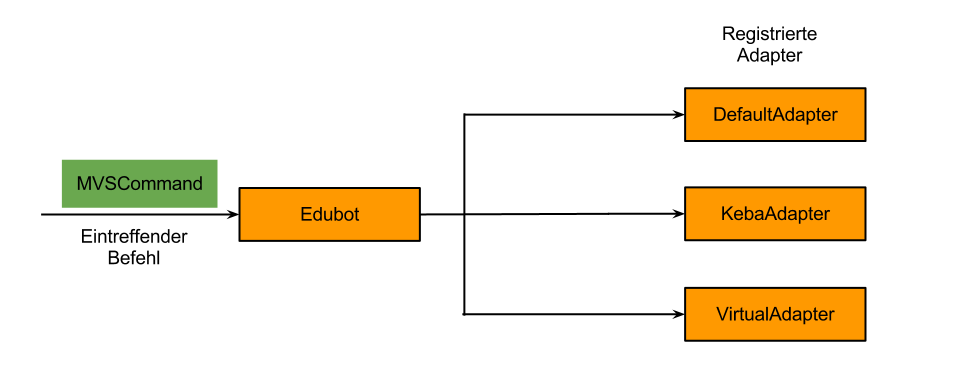
\includegraphics[width=12cm]{images/CommandSystem1} 
    \caption{Ausgangssituation}
  \end{minipage}
\end{figure}
Anschließend wird die \textit{Execute}-Methode der Edubot-Klasse mit einem neuen Befehl aufgerufen, welcher an die registrierten Adapter weitergeleitet wird.
\begin{figure}[H]
  \centering
  \begin{minipage}[t]{12 cm}
  	\centering
  	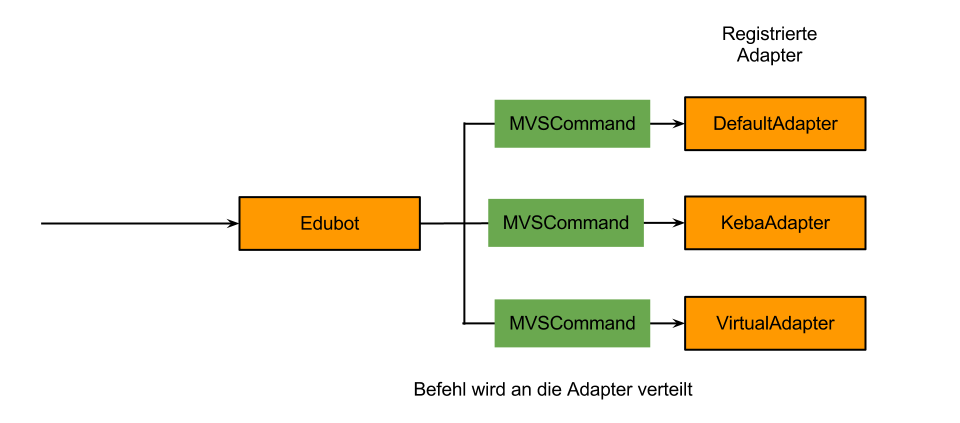
\includegraphics[width=12cm]{images/CommandSystem2} 
    \caption{Eintreffen eines neuen Befehls}
  \end{minipage}
\end{figure}
Das erhaltene Command wird in die Befehlswarteschlangen der Adapter eingereiht. Soll ein Befehl ausgeführt werden, so müssen zuerst die Voraussetzungen dafür überprüft werden. Sind diese erfüllt so werden die entsprechenden Aktionen durchgeführt.
\begin{figure}[H]
  \centering
  \begin{minipage}[t]{12 cm}
  	\centering
  	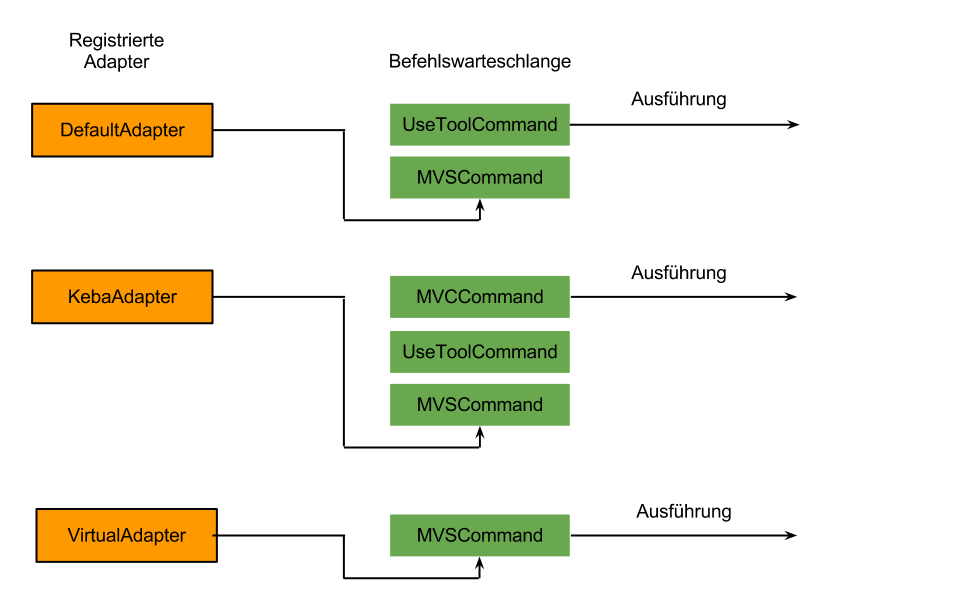
\includegraphics[width=12cm]{images/CommandSystem3} 
    \caption{Warteschlangen-System}
  \end{minipage}
\end{figure}

\subsubsection{Umsetzung}
Das Interface ICommand und die von der API implementierten Befehle werden in den folgenden Abschnitten detailiert beschrieben.

\textbf{ICommand}
\newline
Wie bereits im Aufbau angemerkt, beruht das gesamte System auf dem Interface \textit{IAdapter}, welches den Grundaufbau eines Befehls festlegt. Dieser Aufbau besteht lediglich aus den beiden Methoden "CanExecute" und "Execute".
\begin{itemize}
\item \textbf{CanExecute}
\newline
Bei Aufruf dieser Methode werden die Voraussetzungen für das Ausführen des Befehls mit Hilfe des als Parameter mitgegebenen Adapters geprüft. Sollten die Voraussetzungen nicht erfüllt werden, so wird ein FailureEventArgs-Objekt erzeugt und zurückgegeben. Ist die Überprüfung der Voraussetzungen erfolgreich, so wird \textit{null} zurückgegeben.
\item \textbf{Execute}
\newline
Bei Aufruf dieser Methode werden die von der Art des Befehls abhängigen Aktionen durchführt. Die Methode erhält als Parameter ein Objekt vom Typ \textit{IAdapter}, welches den ausführenden Adapter enthält, wodurch Zugriff auf die Methoden des entsprechenden Adapters gewährleistet ist. Es wird empfohlen die zum Command gehörige Adapter-Methode in einem eigenen Thread zu starten um den Adapter selbst nicht unnötig lange zu blockieren.
\end{itemize}

\textbf{InitCommand}
\newline
Dieser Befehl dient zum Einschalten und Initialisieren des Roboters und stellt im Regelfall den ersten Befehl dar, der an den Roboter geschickt wird. Die \textit{Execute}-Methode ist dabei folgendermaßen implementiert:
\begin{itemize}
\item \textbf{CanExecute}\\
Um eine Initialisierung und das damit verbundene Homing jederzeit zu ermöglichen, gibt diese Methode immer \textbf{true} zurück.
zurückgegeben
\item \textbf{Execute}\\
Bei Aufruf dieser Methode wird das \textit{State}-Property auf \textit{HOMING} gesetzt und das \textit{OnHoming}-Event ausgelöst (mehr dazu im Kapitel Event-System). Zuletzt wird noch ein Thread gestartet, der die \textit{Initialize}-Methode des Adapter ausführt.
\end{itemize}

\textbf{ShutdownCommand}
\newline
Dieser Befehl dient zum Herunterfahren des Roboters und stellt im Regelfall den letzten Befehl dar, der an den Roboter geschickt wird. Die \textit{Execute}-Methode ist dabei folgendermaßen implementiert:
\begin{itemize}
\item \textbf{CanExecute}
\newline
In der CanExecute-Methode wird geprüft ob sich der Adapter im \textit{READY}-Zustand befindet. Sollte sich der Adapter in einem anderen Zustand befinden wird ein FailureEventArgs-Objekt mit einer entsprechenden Nachricht erzeugt und zurückgegeben.
\item \textbf{Execute}
\newline
Bei Aufruf dieser Methode wird das \textit{State}-Property auf \textit{SHUTTING\_DOWN} gesetzt und das \textit{OnShuttingDown}-Event ausgelöst. Zuletzt wird noch ein Thread gestartet, der die \textit{Shutdown}-Methode des Adapter ausführt.
\end{itemize}

\textbf{MVSCommand}
\newline
Dieser Befehl dient zum Verfahren einer linearen Bewegung durch den Roboter. Die \textit{Execute}-Methode ist dabei folgendermaßen implementiert:
\begin{itemize}
\item \textbf{CanExecute}
\newline
In der CanExecute-Methode wird geprüft ob sich der Adapter im \textit{READY}-Zustand befindet. Sollte sich der Adapter in einem anderen Zustand befinden wird ein FailureEventArgs-Objekt mit einer entsprechenden Nachricht erzeugt und zurückgegeben.
\item \textbf{Execute}
\newline
Bei Aufruf dieser Methode wird das \textit{State}-Property auf \textit{MOVING} gesetzt und das \textit{RequiresPrecalculation}-Property des Adapters geprüft. Ist dieser Wert auf \textit{true} gesetzt, so wird der Pfad zum Zielpunkt und die daraus resultierenden Winkelschritte mit Hilfe der InterpolateLinear-Methode der \textit{Interpolation}-Klasse berechnet. Ist die Berechnung erfolgreich, so wird das erzeugte InterpolationResult im Result-Property des Adapters gespeichert. Sollte die Berechnung fehlgeschlagen sein, da zum Beispiel einer der Punkte nicht im gültigen Bereich lag, so wird die Ausführung der Methode mit dem \textit{return}-Schlüsselwort vorzeitig beendet. Im nächsten Schritt wird das  gesetzt und das \textit{OnMovementStarted}-Event ausgelöst. Zuletzt wird noch ein Thread gestartet, der die \textit{MoveStraight}-Methode des Adapter ausführt.
\end{itemize}

\textbf{MVCCommand}
\newline
Dieser Befehl dient zum Verfahren einer zirkularen Bewegung durch den Roboter. Die \textit{Execute}-Methode ist dabei folgendermaßen implementiert:
\begin{itemize}
\item \textbf{CanExecute}
\newline
In der CanExecute-Methode wird geprüft ob sich der Adapter im \textit{READY}-Zustand befindet. Sollte sich der Adapter in einem anderen Zustand befinden wird ein FailureEventArgs-Objekt mit einer entsprechenden Nachricht erzeugt und zurückgegeben.
\item \textbf{Execute}
\newline
Bei Aufruf dieser Methode wird das \textit{State}-Property auf \textit{MOVING} gesetzt und das \textit{RequiresPrecalculation}-Property des Adapters geprüft. Ist dieser Wert auf \textit{true} gesetzt, so wird der Pfad zum Zielpunkt und die daraus resultierenden Winkelschritte mit Hilfe der InterpolateCircular-Methode der \textit{Interpolation}-Klasse berechnet. Ist die Berechnung erfolgreich, so wird das erzeugte InterpolationResult im Result-Property des Adapters gespeichert. Sollte die Berechnung fehlgeschlagen sein, da zum Beispiel einer der Punkte nicht im gültigen Bereich lag, so wird die Ausführung der Methode mit dem \textit{return}-Schlüsselwort vorzeitig beendet. Im nächsten Schritt wird das  gesetzt und das \textit{OnMovementStarted}-Event ausgelöst. Zuletzt wird noch ein Thread gestartet, der die \textit{MoveCircular}-Methode des Adapter ausführt.
\end{itemize}

\textbf{UseToolCommand}
\newline
Dieser Befehl dient zum Aktivieren oder Deaktiveren des verwendeten Werkzeugs. Die \textit{Execute}-Methode ist dabei folgendermaßen implementiert:
\begin{itemize}
\item \textbf{CanExecute}
\newline
In der CanExecute-Methode wird geprüft ob sich der Adapter im \textit{READY}-Zustand befindet. Sollte sich der Adapter in einem anderen Zustand befinden wird ein FailureEventArgs-Objekt mit einer entsprechenden Nachricht erzeugt und zurückgegeben.
\item \textbf{Execute}
\newline
Bei Aufruf dieser Methode wird das \textit{State}-Property auf \textit{MOVING} gesetzt und das \textit{OnToolUsed}-Event ausgelöst. Zuletzt wird noch ein Thread gestartet, der die \textit{UseTool}-Methode des Adapter ausführt. 
\end{itemize}

\textbf{AbortCommand}
\newline
Dieser Befehl dient zum sofortigen Abbruch jeglicher Aktionen die der Roboter im Moment durchführt. Die \textit{Execute}-Methode ist dabei folgendermaßen implementiert:
\begin{itemize}
\item \textbf{CanExecute}
\newline
Da dieser Befehl immer ausgeführt werdne muss, gibt dieser Methode lediglich \textit{true} zurück.
\item \textbf{Execute}
\newline
Bei Aufruf dieser Methode wird die Warteschlange des Roboters geleert um die Gefahr durch nachfolgende Befehle zu eliminieren und das \textit{OnAbort}-Event ausgelöst. Zuletzt wird noch ein Thread gestartet, der die \textit{Abort}-Methode des Adapter ausführt. 
\end{itemize}